\documentclass[10pt,english,aspectratio=169]{beamer}
% Use notes or hide notes or show only notes or handout

\usetheme{default}

\usepackage{xstring}
\usepackage{pgfpages}
%\makeatletter
%\IfSubStr{\@classoptionslist}{handout}
%  {\pgfpagesuselayout{2 on 1}[letterpaper,border shrink=5mm]}
%  {}
%\makeatother

\usepackage{amsmath,amssymb,amsthm}
\usepackage{stmaryrd}
\usepackage{enumerate}
\usepackage{stfloats}
\usepackage{bbm}
\usepackage{pdfpages}
\usepackage{framed}

\usepackage[most]{tcolorbox}
\tcbset{highlight math style={enhanced,
  colframe=white,colback=yellow!15,arc=8pt,boxrule=1pt,
  }}
  
\usepackage{tikz,pgf,pgfplots}
\usepackage{algorithm,algorithmic}
\usepgflibrary{shapes}
\usetikzlibrary{%
  arrows,%
  arrows.meta,
  backgrounds,
  shapes.misc,% wg. rounded rectangle
  shapes.arrows,%
  shapes,%
  calc,%
  chains,%
  matrix,%
  positioning,% wg. " of "
  scopes,%
  decorations.pathmorphing,% /pgf/decoration/random steps | erste Graphik
  shadows,%
  backgrounds,%
  fit,%
  petri,%
  quotes
}

\tikzset{background rectangle/.style={
    fill=white,
  },
  use background/.style={    
    show background rectangle
  }
}

\setbeamersize{text margin left=10mm,text margin right=35mm}

\pgfplotsset{compat=1.12}

%\usetheme{Frankfurt}
%\usecolortheme{ldpc}
\useinnertheme{rounded}
\usecolortheme{whale}
\usecolortheme{orchid}

\newcommand{\ul}[1]{\underline{#1}}
\renewcommand{\Pr}{\mathbb{P}}

%% Setup slides and notes
\makeatletter
\IfSubStr{\@classoptionslist}{notes} { \IfSubStr{\@classoptionslist}{hide} {}{\IfSubStr{\@classoptionslist}{only} {}{\setbeameroption{show notes on second screen=right}}} }{}
\makeatother

\newcommand{\getpdfpages}[2]{\begingroup
  \setbeamercolor{background canvas}{bg=}
  \addtocounter{framenumber}{1}
  \includepdf[pages={#1},%
  pagecommand={%
    \expandafter\def\expandafter\insertshorttitle\expandafter{%
      \insertshorttitle\hfill\insertframenumber\,/\,\inserttotalframenumber}}%
  ]{#2}
  \endgroup}

\newcommand{\backupbegin}{
   \newcounter{finalframe}
   \setcounter{finalframe}{\value{framenumber}}
}
\newcommand{\backupend}{
   \setcounter{framenumber}{\value{finalframe}}
}

 \setbeamercolor{bibliography entry author}{fg=black}
 \setbeamercolor{bibliography entry title}{fg=black}
 \setbeamercolor{bibliography entry location}{fg=black}
 \setbeamercolor{bibliography entry note}{fg=black}
 
 \setbeamerfont{bibliography item}{size=\footnotesize}
 \setbeamerfont{bibliography entry author}{size=\footnotesize}
 \setbeamerfont{bibliography entry title}{size=\footnotesize}
 \setbeamerfont{bibliography entry location}{size=\footnotesize}
 \setbeamerfont{bibliography entry note}{size=\footnotesize}
 \setbeamertemplate{bibliography item}{\insertbiblabel}
 
\newlength\tikzwidth
\newlength\tikzheight


\newcommand{\mc}[1]{\mathcal{#1}}
\newcommand{\mbb}[1]{\mathbb{#1}}
%\newcommand{\expt}{\mbb{E}}
%\newcommand{\dd}{\mathrm{d}}
\newcommand{\Interior}[1]{\ensuremath{{#1}^{\circ}}}
\newcommand{\Closure}[1]{\ensuremath{\overline{#1}}}
\newcommand{\Complement}[1]{\ensuremath{{#1}^{c}}}

\newcommand{\Expect}{\ensuremath{\mathrm{E}}}
\newcommand{\vecnot}{\underline}
\newcommand{\RealNumbers}{\ensuremath{\mathbb{R}}}
\newcommand{\RationalNumbers}{\mathbb{Q}}
\newcommand{\ComplexNumbers}{\mathbb{C}}
\newcommand{\Real}{\mathrm{Re}}
\newcommand{\Span}{\mathrm{span}}
\newcommand{\Rank}{\mathrm{rank}}
\newcommand{\Nullity}{\mathrm{nullity}}
\newcommand{\Trace}{\mathrm{tr}}
\newcommand{\Diag}{\mathrm{diag}}
\newcommand{\dd}{\mathrm{d}}
\DeclareMathOperator*{\esssup}{ess\,sup}

% Use < , > inner product
\newcommand{\inner}[2]{{\left\langle #1 \mskip2mu , #2 \right\rangle}}
\newcommand{\tinner}[2]{{\langle #1 \mskip1mu , #2 \rangle}}

% Use < | > inner product
%\newcommand{\inner}[2]{{\left\langle #1 \mskip2mu \middle| \mskip2mu #2 \right\rangle}}
%\newcommand{\tinner}[2]{{\langle #1 \mskip1mu | \mskip1mu  #2 \rangle}}




\def\checkmark{\tikz\fill[scale=0.4](0,.35) -- (.25,0) -- (1,.7) -- (.25,.15) -- cycle;}
\def\greencheck{{\color{green}\checkmark}}
\def\scalecheck{\resizebox{\widthof{\checkmark}*\ratio{\widthof{x}}{\widthof{\normalsize x}}}{!}{\checkmark}}
\def\xmark{\tikz [x=1.4ex,y=1.4ex,line width=.2ex, red] \draw (0,0) -- (1,1) (0,1) -- (1,0);}
\def\redx{{\color{red}\xmark}}

\renewcommand{\footnotesep}{-2pt}


\begin{document}



\title{ECE 586: Vector Space Methods \\ Lecture 8 Flip Video: Compactness}
\author{Henry D. Pfister \\ Duke University}
\date{}
%\date{August 20th, 2020}
%\maketitle

\setbeamertemplate{navigation symbols}{}

\begin{frame}[plain]
	\titlepage
	
	\note{
		\vspace{8mm}
		\begin{enumerate}
			\setlength\itemsep{3mm}
			\color{red}
			\item Welcome to the eighth video lecture for ECE 586, Vector Space Methods. \\[2mm]
			Today, we'll discuss the idea of compactness and its applications.
		\end{enumerate}
	}
\end{frame}

\addtocounter{framenumber}{-1}
\setbeamertemplate{navigation symbols}{\textcolor{blue}{\footnotesize \insertframenumber ~/ \inserttotalframenumber}}


\begin{frame}<beamer:1-7 | handout:1-5>
\frametitle{2.1.4: Compactness}

\begin{definition}<1->
A metric space $(X,d)$ is \textcolor{blue}{totally bounded} if, for any $\epsilon > 0$, there exists a finite set of radius-$\epsilon$ balls that cover $X$ (i.e., $\cup_{x\in S} B_d (x,\epsilon) = X$).
\end{definition}

\begin{definition}<beamer:5-|handout:3->
A metric space is \textcolor{blue}{compact} if it is complete~and~totally~bounded.
\end{definition}

\begin{itemize}
\setlength\itemsep{3mm}
\item<beamer:6-|handout:4-> Examples \vspace{1mm}
\begin{itemize} 
  \setlength\itemsep{1.5mm}
  \item The closed real interval $[0,1]\subset \RealNumbers$ is compact
  \item A subset of Euclidean $\RealNumbers^n$ is compact iff it is closed and bounded
  \item But, the standard metric space of real numbers is not compact because it is not totally bounded.
\end{itemize}

\end{itemize}

\begin{theorem}<beamer:7|handout:5>
A closed subset $A$ of a compact space $X$ is itself a compact space.
\end{theorem}

\uncover<beamer:2-5|handout:2-3>{%
\begin{tikzpicture}[overlay,remember picture,shift={(10.75,1.25)}]
\draw[fill=brown!30,rounded corners] (-1.3,-0.9) rectangle (4.1,3.15);

\only<beamer:2-5|handout:2-3>{%
\draw[very thick,fill=white] (-0.5,-0.4) rectangle (3.35,2.6);
}

\only<beamer:2|handout:0>{%
\node at (2.6,2.2) {$X \subset\mathbb{R}^2$};
}

\only<beamer:3|handout:2-3>{%
\begin{scope}[shift={(-0.08,0.1)}]
%\clip (-0.4,-0.5) rectangle (3.45,2.5);
\foreach \x in {0,1,2,3}
  \foreach \y in {0,1,2}
    \draw[thick,blue!70,fill=gray,fill opacity=0.2] (\x,\y) circle (0.72);
\end{scope}
}

\only<beamer:4-5|handout:0>{%
\begin{scope}[shift={(-0.32,-0.16)}]
%\clip (-0.4,-0.5) rectangle (3.45,2.5);
\foreach \x in {0,0.5,1,1.5,2,2.5,3,3.5}
  \foreach \y in {0,0.5,1,1.5,2,2.5}
    \draw[thick,blue!70,fill=gray,fill opacity=0.2] (\x,\y) circle (0.36);
\end{scope}
}

\end{tikzpicture}
}

\note{
	\vspace{2mm}
	\begin{enumerate}[<alert@+>]
		\footnotesize
		\setlength\itemsep{3mm}
		\item Compactness is a very useful property in analysis that identifies when an arbitrary metric space behaves (in some sense) like a closed and bounded subset of real numbers. \\[3mm]
		Read
		\item For example, let $X$ be this subset of $\mathbb{R}^2$.
		\item For some positive $\epsilon$, we can cover this set by a finite number of radius $\epsilon$ balls.
		\item Reducing $\epsilon$, we can repeat this.  In fact, we can do this for any $\epsilon > 0$.  Thus, $X$ is totally bounded.
		\item Read.  We will see that compactness plays an important role in the convergence of sequences.
		\item Read.  This is because $N$ balls of radius $\epsilon$ can cover a width of at most $N\epsilon$.
		\item Read.  As an exercise, think about how you might prove this.
	\end{enumerate}
}

\end{frame}

\begin{frame}<1-3>
\frametitle{2.1.4: Compactness and Sequences}

\begin{definition}<1->
Let $x_1,x_2,\ldots \in X$ be a sequence and $n_1,n_2,\ldots\in \mathbb{N}$ be
a strictly increasing sequence (i.e., $n_{i+1}>n_i$).
Then, $x_{n_k} = (x_{n_1},x_{n_2},\ldots)$ is a \textcolor{blue}{subsequence} of $x_n$.
\end{definition}

\begin{theorem}<2->[Bolzano--Weierstrass]
A sequence in a compact metric space has a subsequence that converges.
\end{theorem}

\begin{example}<3->
For the compact metric space $X=[-2,2]\subset \mathbb{R}$ with absolute distance, let $x_n = (-1)^n + \frac{1}{n}$.
Then, the subsequence $x_2,x_4,x_6,\ldots$ converges to 1.
\end{example}

\begin{itemize}
\item<3-> Does the sequence $x_n$ have any other limit points?
\end{itemize}

\note{
	\vspace{2mm}
	\begin{enumerate}[<alert@+>]
		\footnotesize
		\setlength\itemsep{3mm}
		\item Read.
		\item Read. This property is used somewhat regularly in analysis.
		\item Read. This is because $-1$ to an even power equals 1 and $1/n$ vanishes as $n\to \infty$.  \\ [3mm] Read. Consider the subsequence $x_1,x_3,x_5,\ldots$.  Does this converge?
	\end{enumerate}
}

\end{frame}



\begin{frame}<1-7>
\frametitle{2.1.4: Bolzano--Weierstrass for a Closed Real Interval}

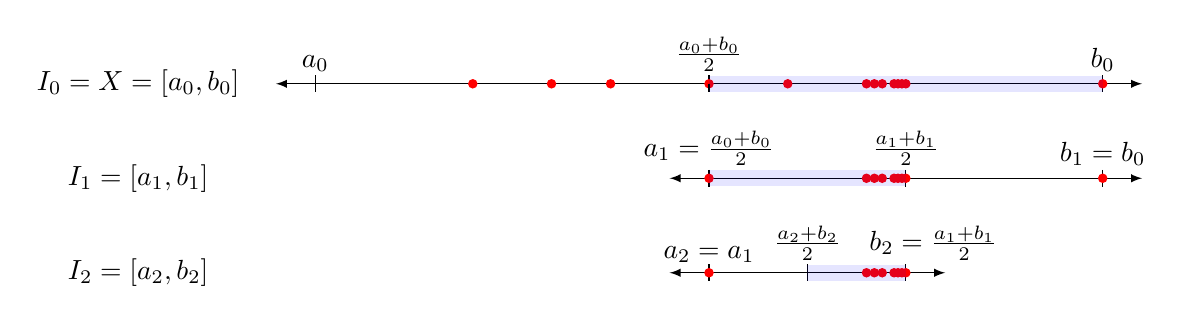
\begin{tikzpicture}

\node at (-7.25,0) {$I_0 = X = [a_0,b_0]$};
\draw[latex-latex] (-5.5,0) -- (5.5,0) ; %edit here for the axis
\foreach \x in {-5,0,5}
  \draw[shift={(\x,0)},color=black] (0pt,3pt) -- (0pt,-3pt);
\draw[shift={(-5,0)},color=black] (0pt,0pt) -- (0pt,-3pt) node[above,yshift=4] 
{$a_0$};
\draw[shift={(5,0)},color=black] (0pt,0pt) -- (0pt,-3pt) node[above,yshift=4] 
{$b_0$};
\foreach \x in {-3,-2,-1.25,1,0,2,2.1,2.2,2.35,2.4,2.45,2.5,5}
  \draw[shift={(\x,0)},color=red,fill] (0,0) circle (1.5pt);

\uncover<2->{%
\draw[shift={(0,0)}] (0pt,0pt) -- (0pt,-3pt) node[above,yshift=4] 
{$\frac{a_0+b_0}{2}$};
}

\uncover<3->{%
\draw[draw=none,fill=blue,opacity=0.1] (0,-0.1) rectangle (5,0.1);
}

\uncover<4->{%

\begin{scope}[yshift=-1.2cm]
\node at (-7.25,0) {$I_1 = [a_1,b_1]$};
\draw[latex-latex] (-0.5,0) -- (5.5,0) ; %edit here for the axis
\foreach \x in {0,2.5,5}
  \draw[shift={(\x,0)},color=black] (0pt,3pt) -- (0pt,-3pt);
\draw[shift={(0,0)},color=black] (0pt,0pt) -- (0pt,-3pt) node[above,yshift=4] 
{$a_1 = \frac{a_0+b_0}{2}$};
\draw[shift={(5,0)},color=black] (0pt,0pt) -- (0pt,-3pt) node[above,yshift=4] 
{$b_1=b_0$};
\draw[shift={(2.5,0)},color=black] (0pt,0pt) -- (0pt,-3pt) node[above,yshift=4] 
{$\frac{a_1+b_1}{2}$};
\foreach \x in {0,2,2.1,2.2,2.35,2.4,2.45,2.5,5}
  \draw[shift={(\x,0)},color=red,fill] (0,0) circle (1.5pt);
\end{scope}
}


\uncover<5->{%
\draw[draw=none,fill=blue,opacity=0.1] (0,-1.3) rectangle (2.5,-1.1);
}

\uncover<6->{%

\begin{scope}[yshift=-2.4cm]
\node at (-7.25,0) {$I_2 = [a_2,b_2]$};
\draw[latex-latex] (-0.5,0) -- (3,0) ; %edit here for the axis
\foreach \x in {0,1.25,2.5}
  \draw[shift={(\x,0)},color=black] (0pt,3pt) -- (0pt,-3pt);
\draw[shift={(0,0)},color=black] (0pt,0pt) -- (0pt,-3pt) node[above,yshift=3] 
{$a_2 = a_1$};
\draw[shift={(2.5,0)},color=black] (0pt,0pt) -- (0pt,-3pt) node[above,xshift=10,yshift=4] 
{$b_2 = \frac{a_1+b_1}{2}$};
\draw[shift={(1.25,0)},color=black] (0pt,0pt) -- (0pt,-3pt) node[above,yshift=4] 
{$\frac{a_2+b_2}{2}$};
\foreach \x in {0,2,2.1,2.2,2.35,2.4,2.45,2.5}
  \draw[shift={(\x,0)},color=red,fill] (0,0) circle (1.5pt);
\end{scope}

\draw[draw=none,fill=blue,opacity=0.1] (1.25,-2.3) rectangle (2.5,-2.5);

}

\end{tikzpicture}
\vspace{-3mm}

\begin{itemize}
\setlength{\itemsep}{1.25mm}
\item<1-> For $X = [a_0,b_0] \subseteq \mathbb{R}$ with $d(x,y) = |x-y|$, let $x_n^{(0)} \in X$ be the red dots$\!\!\!\!\!\!\!\!\!$
\item<2-> Observe \textcolor{blue}{$|\{n\in \mathbb{N} \, |\, x_{n}^{(0)} \in I_0 \} | = \infty$} and split interval $I_0$ in half at $\frac{a_0+b_0}{2}$
\item<3-> Of the two halves, \textcolor{blue}{at least one must contain infinitely many elements of $x_n^{(0)}\!\!\!\!\!\!$}
\item<4-> \mbox{Call it $I_1$ and let $x_{n}^{(1)}$ be the subseq of $x_n^{(0)}$ in $I_1$. Then, $|\{n\in \mathbb{N} \, |\, x^{(1)}_{n} \in I_1 \} | = \infty\!\!\!\!\!\!\!\!\!\!\!\!\!\!\!\!\!\!\!\!\!\!\!\!\!\!\!$}
\item<5-> Of the two halves of $I_1$, \textcolor{blue}{one must contain infinitely many elements of $x_n^{(1)}$}
\item<6-> Continuing by induction, the \textcolor{blue}{length of $I_k$ is $|b_k-a_k| = 2^{-k}| b_0-a_0 |$}
\item<7-> Using this, one can show $x^{(k)}_k$ is a  \textcolor{blue}{subsequence} of $x_n$ that is \textcolor{blue}{Cauchy}
\end{itemize}

\note{
	\vspace{2mm}
	\begin{enumerate}[<alert@+>]
		\footnotesize
		\setlength\itemsep{3mm}
		\item Now, we will outline the proof of the Bolzano--Weierstrass Theorem. \\ [3mm] Read.
		\item Read.
		\item Read.  In the example, this is the right half and it is highlighted.
		\item Read.
		\item Read.
		\item Now, we can see the pattern and proceed by induction.  After $k$ steps, this shows that... Read.
		\item The $k$-th subsequence, $x^{(k)}_n \in I_k$, has all elements within distance $2^{-k}|b_0 - a_0|$.
		\item Thus, the diagonal sequence $x^{(k)}_k$ is a subsequence Cauchy.  Why can't we pick $x^{(k)}_1$ instead?
	\end{enumerate}
}

\end{frame}


\begin{frame}<1-3>
\frametitle{2.1.5: Two Important Consequences}

\begin{theorem}<1->
Let $X$ be a metric space and $f \colon X\rightarrow \RealNumbers$ be a continuous function from $X$ to $\mathbb{R}$.
If $A$ is a compact subset of $X$, then there exists $x\in A$ such that $f(x)=\sup f(A)$ (i.e., $f$ achieves a maximum on $A$).
\end{theorem}

\vspace{3mm}

\begin{theorem}<2->
Let $(X,d)$ be a compact metric space and $C(X)$ be the set of continuous functions mapping $X$ to $\mathbb{R}$.
This set of functions, with the metric \vspace{-1.5mm} \[d_\infty (f,g) \triangleq \sup_{x\in X} |f(x)-g(x)| = \max_{x\in X} |f(x)-g(x)|, \vspace*{-1.5mm}\] defines a complete metric space.
\end{theorem}

\uncover<3->{Note: For $f,g\in C(X)$, $d_\infty$ metrizes uniform convergence because \vspace{-1.5mm} \[ \text{``}\max_{x\in X} |f(x)-g(x)| < \epsilon \text{''} \Leftrightarrow \text{``} \forall x\in X, |f(x) - g(x)| < \epsilon \text{''}. \]}

\note{
	\vspace{2mm}
	\begin{enumerate}[<alert@+>]
		\footnotesize
		\setlength\itemsep{3mm}
		\item Read. This result is often summarized as ``A continuous function on a compact set achieves a maximum value''.
		\item The previous result allows one to define a complete metric space of functions... Read.
		\item We say that a metric ``metrizes'' a type of convergence if convergence under that metric is equivalent to that type of convergence.
	\end{enumerate}
}

\end{frame}


\begin{frame} \frametitle{Next Steps}

\begin{itemize}
\setlength\itemsep{5mm}
\item To continue studying after this video -- \vspace{2mm}

\begin{itemize}
 \setlength\itemsep{3mm}
 \item Try the suggested reading: Course Notes EF 2.1.4 - 2.1.5
 \item Or the optional reading: MMA 2.1
 \item Also, look at the problems in Assignment 3
\end{itemize}
\end{itemize}

\note{
	\vspace{8mm}
	\begin{enumerate}
		\setlength\itemsep{3mm}
		\color{red}
		\item Here are some options to continue learning this material. (read) \\ [2mm]  That's it for today.  So, I'll see you next time.
	\end{enumerate}
}

\end{frame}


\end{document}

  
\backupbegin

%\begin{frame}
%\frametitle{Backup Slides}
%\begin{itemize}
%\item Slide numbers not included in denominator!
%\end{itemize}
%\end{frame}

%\begin{frame}[allowframebreaks]
%\frametitle{References}
%\bibliographystyle{alpha}
%\footnotesize
%\bibliography{IEEEabrv,WCLabrv,WCLbib,WCLnewbib}
%\end{frame}

\backupend

\end{document}
